%%%%%%%%%%%%%%%%%%%%%%%%%%%%%%%%%%%%%
%
% rogue2019.tex
%
% (c) Rogue Robotics 2018
%
% Source file for technical documentation
% See roguedoc.cls file for more
%
%%%%%%%%%%%%%%%%%%%%%%%%%%%%%%%%%%%%%

\documentclass{roguedoc}

% setup our nice math styling
\usepackage{amsmath}
\usepackage{amssymb}
\usepackage{unicode-math}
\setmathfont{Latin Modern Math}
\renewcommand{\vec}[1]{\mathbf{#1}}

% basic document info
\title{2019 Technical Report}
\author{Rogue Robotics Club}
\setcopyright{This document and associated \LaTeX{} template are (c) Rogue Robotics.}

\begin{document}
\roguetoc{}

\section{Stuff}
Here is some placeholder content. It is obviously very advanced math. Here, have a Gaussian integral:
\begin{equation}
  \int _{-\infty} ^{a} \frac{1}{\sqrt{2\pi}} e^{x^2/2}\,dx
\end{equation}

\section{Also Stuff}
Here is some \emph{more} placeholder content!

\section{Even More Stuff}
Well, there's even more stuff here!

\section{Propulsion}
\emph{Alice}'s six Blue Robotics T100 thrusters were reused from last year. Compared to bilge pump motors with which team members had worked in the past, the T100s have superior thrust characteristics and power efficiency. In order to design efficient control algorithms and thruster mappings, the company mathematically modeled the vehicle dynamics with a three-dimensional rigid-body analysis.

\begin{figure}[H]
  \centering
  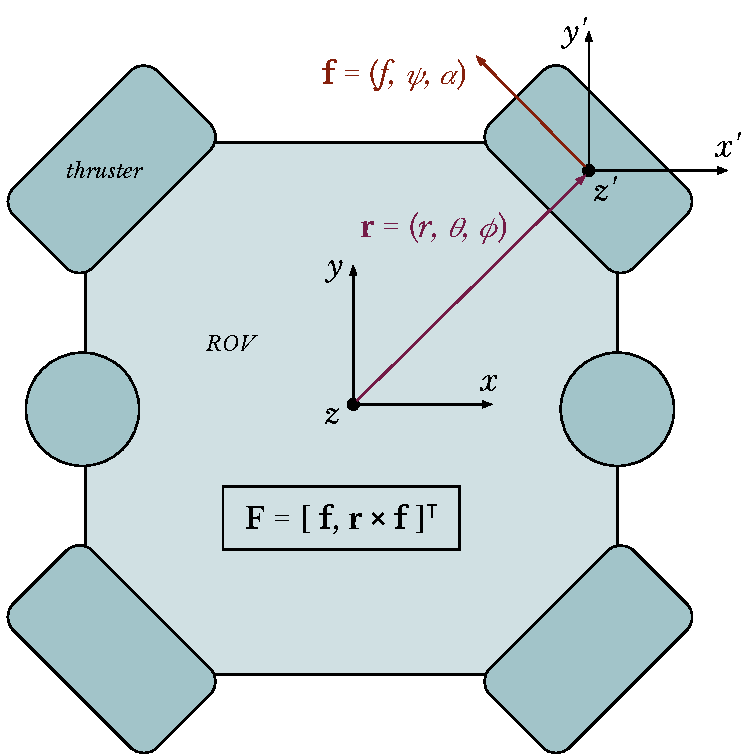
\includegraphics[width=0.5\textwidth]{img/thruster_mapping.pdf}
  \caption{Rigid-body model of an ROV under the influence of a thrust $\vec{f}$ at a thruster located at $\vec{r}$.}
\end{figure}

The relationship between the vector of thruster forces $\vec{f}$ is related to the net forces and torques on the ROV $\vec{F}$ by $\vec{F} = \Lambda\vec{f}$, where the structure matrix is:
\begin{equation}
  \Lambda =
    \begin{bmatrix}
      \sin\psi_i\cos\alpha_i \\
      \sin\psi_i\sin\alpha_i \\
      \cos\psi_i \\
      r_i\sin\theta_i\sin\phi_i\cos\psi_i - r_i\cos\theta_i\sin\psi_i\sin\alpha_i \\
      r_i\cos\theta_i\sin\psi_i\cos\alpha_i - r_i\sin\theta_i\cos\phi_i\cos\psi_i \\
      r_i\sin\theta_i\sin\psi_i\sin(\alpha_i-\phi_i)
    \end{bmatrix}
\end{equation}

\end{document}
